\documentclass{sjtuarticle}
\graphicspath{{figs/}}
\usepackage{booktabs}
\let\Bbbk\relax
\usepackage[citations,fencedCode,underscores=false]{markdown}
\usepackage[style=gb7714-2015]{biblatex}
\addbibresource{ref.bib}
\usepackage[colorlinks]{hyperref}
\newcommand{\file}[1]{\textsf{#1}}
\title{基于 ReLM 模型的中文拼写纠错}
\author{LogCreative}
\date{2024年5月25日}
\begin{document}
\maketitle
\begin{abstract}
    本文基于 ReLM 模型对 MAK 数据集进行中文拼写纠错,在测试集上达到 68.18\% 的准确率。
\end{abstract}
\tableofcontents*
\clearpage
\section{数据集}\label{sec:dataset}
MAK中文拼写纠错数据集语料内容相近于小红书软件的说话风格,相较于普通的中文语料而言,其语料中包含有较多的自造词(“集美”、“一下子就看会惹”),这些自造词由于大概率不在词典中可能会被误判为错字,但是在该数据集环境下实际上是正确的中文表达,这是在该数据集上取得良好效果的一大挑战。

MAK数据集包含两个部分:训练数据 \file{train\_data.tsv} 有5000条输入输出对,测试文件 \file{test\_data.tsv} 有200条输入数据。本文将训练数据按照 9:1 的比例顺序划分为训练集 \file{train\_data\_2.tsv}(4500条) 和验证集 \file{dev\_data\_2.tsv}(500条)。
\section{模型介绍}

\subsection{BERT}

近年来,基于注意力机制的模型,特别是 Transformer\cite{transformer},由于可以训练出长距离的依赖信息、相较于普通的循环神经网络(Recurrent Neural Network, RNN)更加并行,而成为自然语言处理领域具有革命性的一派。
其中,BERT (Bidirectional Encoder Representations from Transformers)\cite{bert} 基于 Transformer 通过上下文双向预测大幅改善了自然语言处理领域先在大数据集上预训练、再在特定数据集上微调方法(即 pretrain--finetune)于语言任务中的效果。

如图 \ref{fig:bert} 所示,BERT 的输入是以分隔符分开的文本序列,输入序列可以是一句话,也可以是多
个句子。每个输入序列开头使用一个特殊的\verb"[CLS]"符号进行标记,每句的句尾
用标识符\verb"[SEP]"以标识和分隔不同句子。这里的\verb"[CLS]"符号在经过BERT 编
码后能起到作为整个输入序列的上下文表示的效果\cite{nlp}。

\begin{figure}[h]
    \centering
    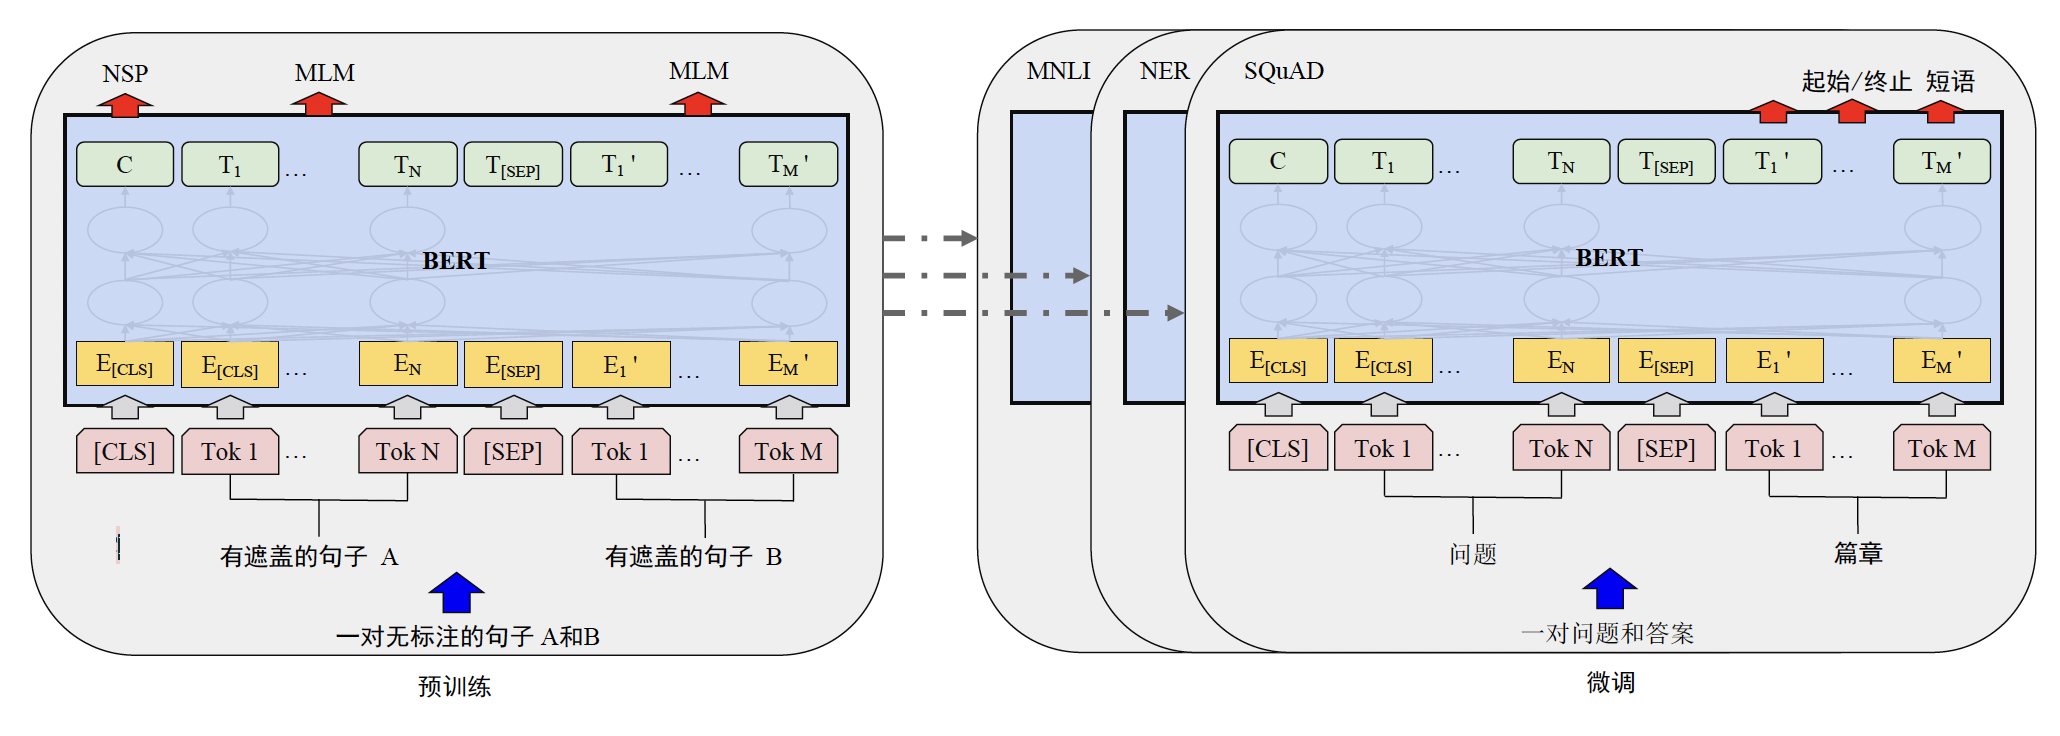
\includegraphics[width=0.9\textwidth]{bert.png}
    \caption{BERT 结构图\cite{nlp}}
    \label{fig:bert}
\end{figure}

bert-base-chinese \cite{bertc}是谷歌官方基于中文语料库的 BERT 预训练模型。

\subsection{ReLM}
ReLM (Rephrasing Language Model) \cite{relm} 提出了新的纠错训练目标“重述语言模型”,相较于 BERT-Tagging,尽可能减少模型对于词对记忆的过拟合现象,并尽可能通过语义层面对错别字进行修正。

如图 \ref{fig:relm} 所示,基于 BERT,ReLM 给出了一种非自回归(non-auto-regressive)的实现,相较于自回归中使用 \verb"[EOS]" 来标识句子结束,ReLM不使用该标识符号而是采用 $\{x_1,\cdots,x_n,\langle\text{sep}\rangle,m_1,\cdots,m_n,\langle\text{sep}\rangle\}$ 强制模型输出相同字符数目的文本。为了进一步减少学习到词对的可能性,并增加理解语义的可能,还会对输入随机遮掩,使得输入进一步变为 $\{x_1,\cdots,m_i^\prime,\cdots,\langle\text{sep}\rangle,m_1,\cdots,m_n,\langle\text{sep}\rangle\}$。

\begin{figure}[h]
    \centering
    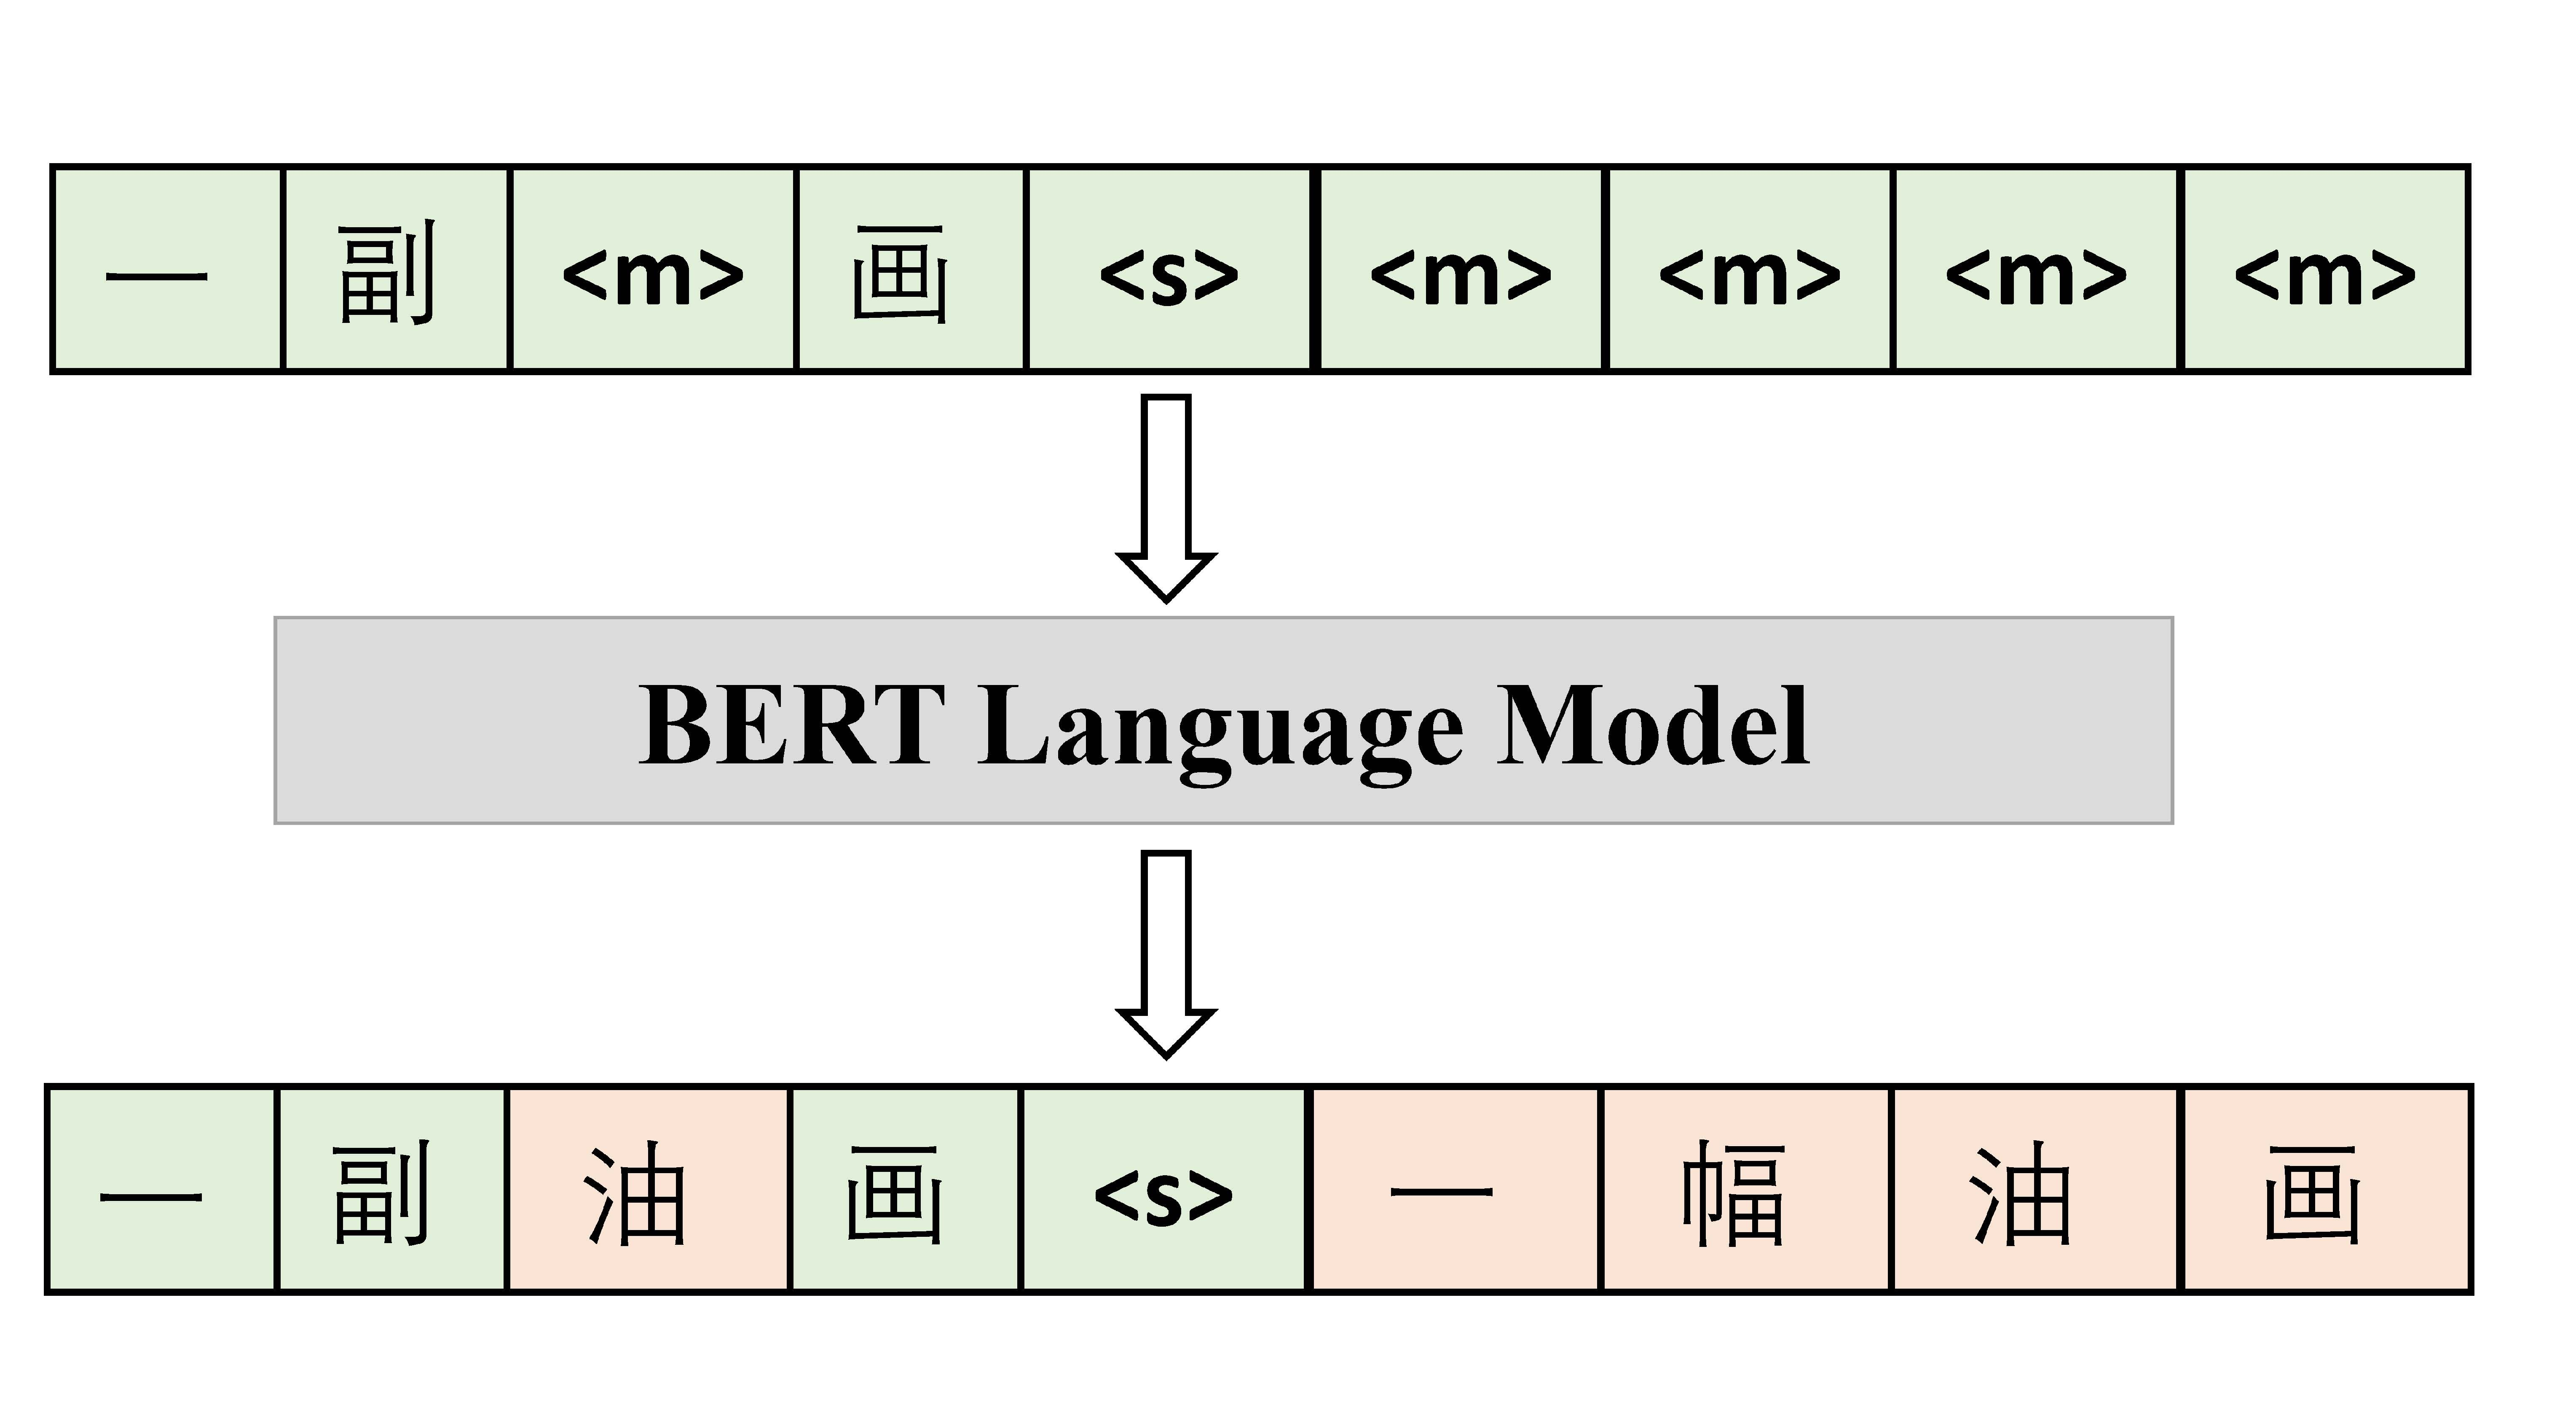
\includegraphics{relm.jpg}
    \caption{ReLM 的输入输出}
    \label{fig:relm}
\end{figure}

\section{模型选择与评估}

正如第 \ref{sec:dataset} 节指出的,如果直接使用普通的ReLM预训练模型对MAK测试集进行推理,可能会对专有名词有很多的误判。因此,本文通过使用训练集 \file{train\_data\_2.tsv} 对 ReLM 预训练模型(基于 bert-base-chinese 并已在 3400 万中文语料上微调的预训练模型)进行微调,并在验证集 \file{dev\_data\_2.tsv} 上进行验证。

本文也尝试使用 Qwen1.5-7b \cite{qwen} 作为基础模型使用 SFT 的方式进行基准实验。

验证集主要使用 $F_1$ 分数作为判断标准,它是精确率$P$(预测为正的样本中有多少是真正的正样本)和召回率$R$(样本中的正例有
多少被正确预测了)的调和平均数:
\begin{equation}
    F_1=\frac{2RP}{R+P}
\end{equation}

测试集将使用 Kaggle 评测系统\cite{kaggle}得出准确率分数\footnote{由于写作时比赛尚未结束,所以该结果只基于 33\% 的测试集。}。

\section{性能分析}

\subsection{实验设置}

实验操作系统为 Ubuntu 22.04,GPU 为 Nvidia A100 80G,CUDA 版本为 11.8。

对 ReLM 微调时,批量大小(batch size)为 128,AdamW 优化器初始学习率为 $1\times 10^{-5}$,预热比例(warmup proportion)为 0.06,权重衰减(weight decay)为0,随机遮掩噪音概率(noise probability)为0.2。在没有特殊说明的情况下使用 fp16 混合精度,每隔100个轮次(epoch)验证并保存模型,最大1000轮次。

对 Qwen1.5-7b 微调时,批量大小为1,AdamW 优化器初始学习率为 $3\times 10^{-5}$,预热比例(warmup proportion)为 0.06,权重衰减(weight decay)为0,最大3轮次。采用 fp16 混合精度。LoRA 配置\cite{qwensft}为 \begin{verbatim}
    LoraConfig(
        r=8,
        lora_alpha=16,
        target_modules=["q_proj","k_proj","v_proj",
            "gate_proj", "down_proj", "up_proj"],
        lora_dropout=0.1,
        bias="none",
        task_type="CAUSAL_LM",
    )
\end{verbatim}

\subsection{实验结果}

如表 \ref{tab:relmres} 所示,ReLM 在随机种子为 1024 的情况下,学习率我为$1\times 10^{-5}$,800轮训练后在验证集上达到 92.20\% 的 $F_1$ 分数,在(33\% 的)测试集上达到 68.18\% 的准确率。

\begin{table}[h]
    \centering
    \caption{实验结果}
    \label{tab:relmres}
    \begin{tabular}{cccccccc}
        \toprule
        序号 & 模型  & $\frac{\text{训练集}}{\text{验证集}}$ & 随机种子 & 初始学习率 &  训练轮数 & 验证集 $F_1$ (\%) & 测试集准确率 (\%) \\
        \midrule
        0 & ReLM+BERT & 9:1 & -- & -- & -- & 25.46 & 43.94 \\
        1 & ReLM+BERT & 9:1 & 42 & $5\times10^{-5}$ & 400 & 90.95 & 63.64 \\
        2 & ReLM+BERT & 9:1 & 2024 &$5\times10^{-5}$ &  400 & 90.72 & 65.15 \\
        3 & ReLM+BERT & 9:1 & 1024 &$5\times10^{-5}$ &  500 & 91.04 & 66.67 \\
        4 & ReLM+BERT & 9:1 & 1024 &$1\times10^{-5}$ &  800 &  92.20 & \bfseries 68.18 \\
        5 & ReLM+BERT & 9:1 & 1024 & $5\times10^{-6}$ & 1700 & \bfseries 93.13 & 63.64 \\
        \midrule
        6 & ReLM+BERT & 4:1  & 42 & $5\times10^{-5}$ & 600 & 89.43 & 62.12\\
        7 & ReLM+BERT & 24:1 & 1024 & $5\times10^{-5}$ & 100 & 92.58 & 63.64 \\
        8 & ReLM+BERT (fp32) & 9:1 & 1024 & $5\times10^{-5}$ & 300 & 91.04 & 62.12 \\
        \midrule
        9 & Qwen1.5-7b & 9:1 & 1024 & $3\times10^{-5}$ & 3 & $P=60.00$\footnotemark[1] & 28.79 \\
        \bottomrule
    \end{tabular}
\end{table}
\footnotetext[1]{仅为句子准确率。}

\subsection{参数选择}

\paragraph{训练集/验证集划分比例}

训练集越多,可用于训练的语料也就越多,但与此同时,验证集也就越少,模型验证时的准确率会有波动,影响对模型性能的判断。比较实验 1、6、7,可以看到9:1是一个比较适中的比例:4:1没有足够多的训练数据;24:1验证集过小,即使在验证集上拥有较好的性能,却没能在测试集上拥有较好的性能。

\paragraph{随机种子}

由于“随机遮掩”用到了随机种子,所以随机种子也会对性能造成一定的影响。

\paragraph{初始学习率}

初始学习率过大时,会导致跳过最优点的情况;初始学习率过小,会导致训练过程过慢,有时甚至到不了最优点。比较实验3、4、5,可以看到 $1\times 10^{-5}$ 是合适的学习率,更小时虽然在验证集上拥有更高的分数,但是在测试集上未必有更好的效果。

\paragraph{训练轮数}

本文采用当前配置中 $F_1$ 性能最高的对应轮数提交。

\paragraph{模型精度} 大部分都使用了 fp16 混合精度,对比3和8,可以看到使用原始精度fp32并不一定带来效果上的提升,而且训练时长和训练需要的显存大约增加了一倍。

\section{结论}

本文基于 ReLM 对 MAK 中文拼写纠错数据集进行实验,通过调整训练集/验证集划分比例、随机种子、初始学习率,最终得到在随机种子为 1024 的情况下,学习率我为$1\times 10^{-5}$,800轮训练后在测试集上达到 68.18\% 的准确率。

\begin{figure}[h]
    \centering
    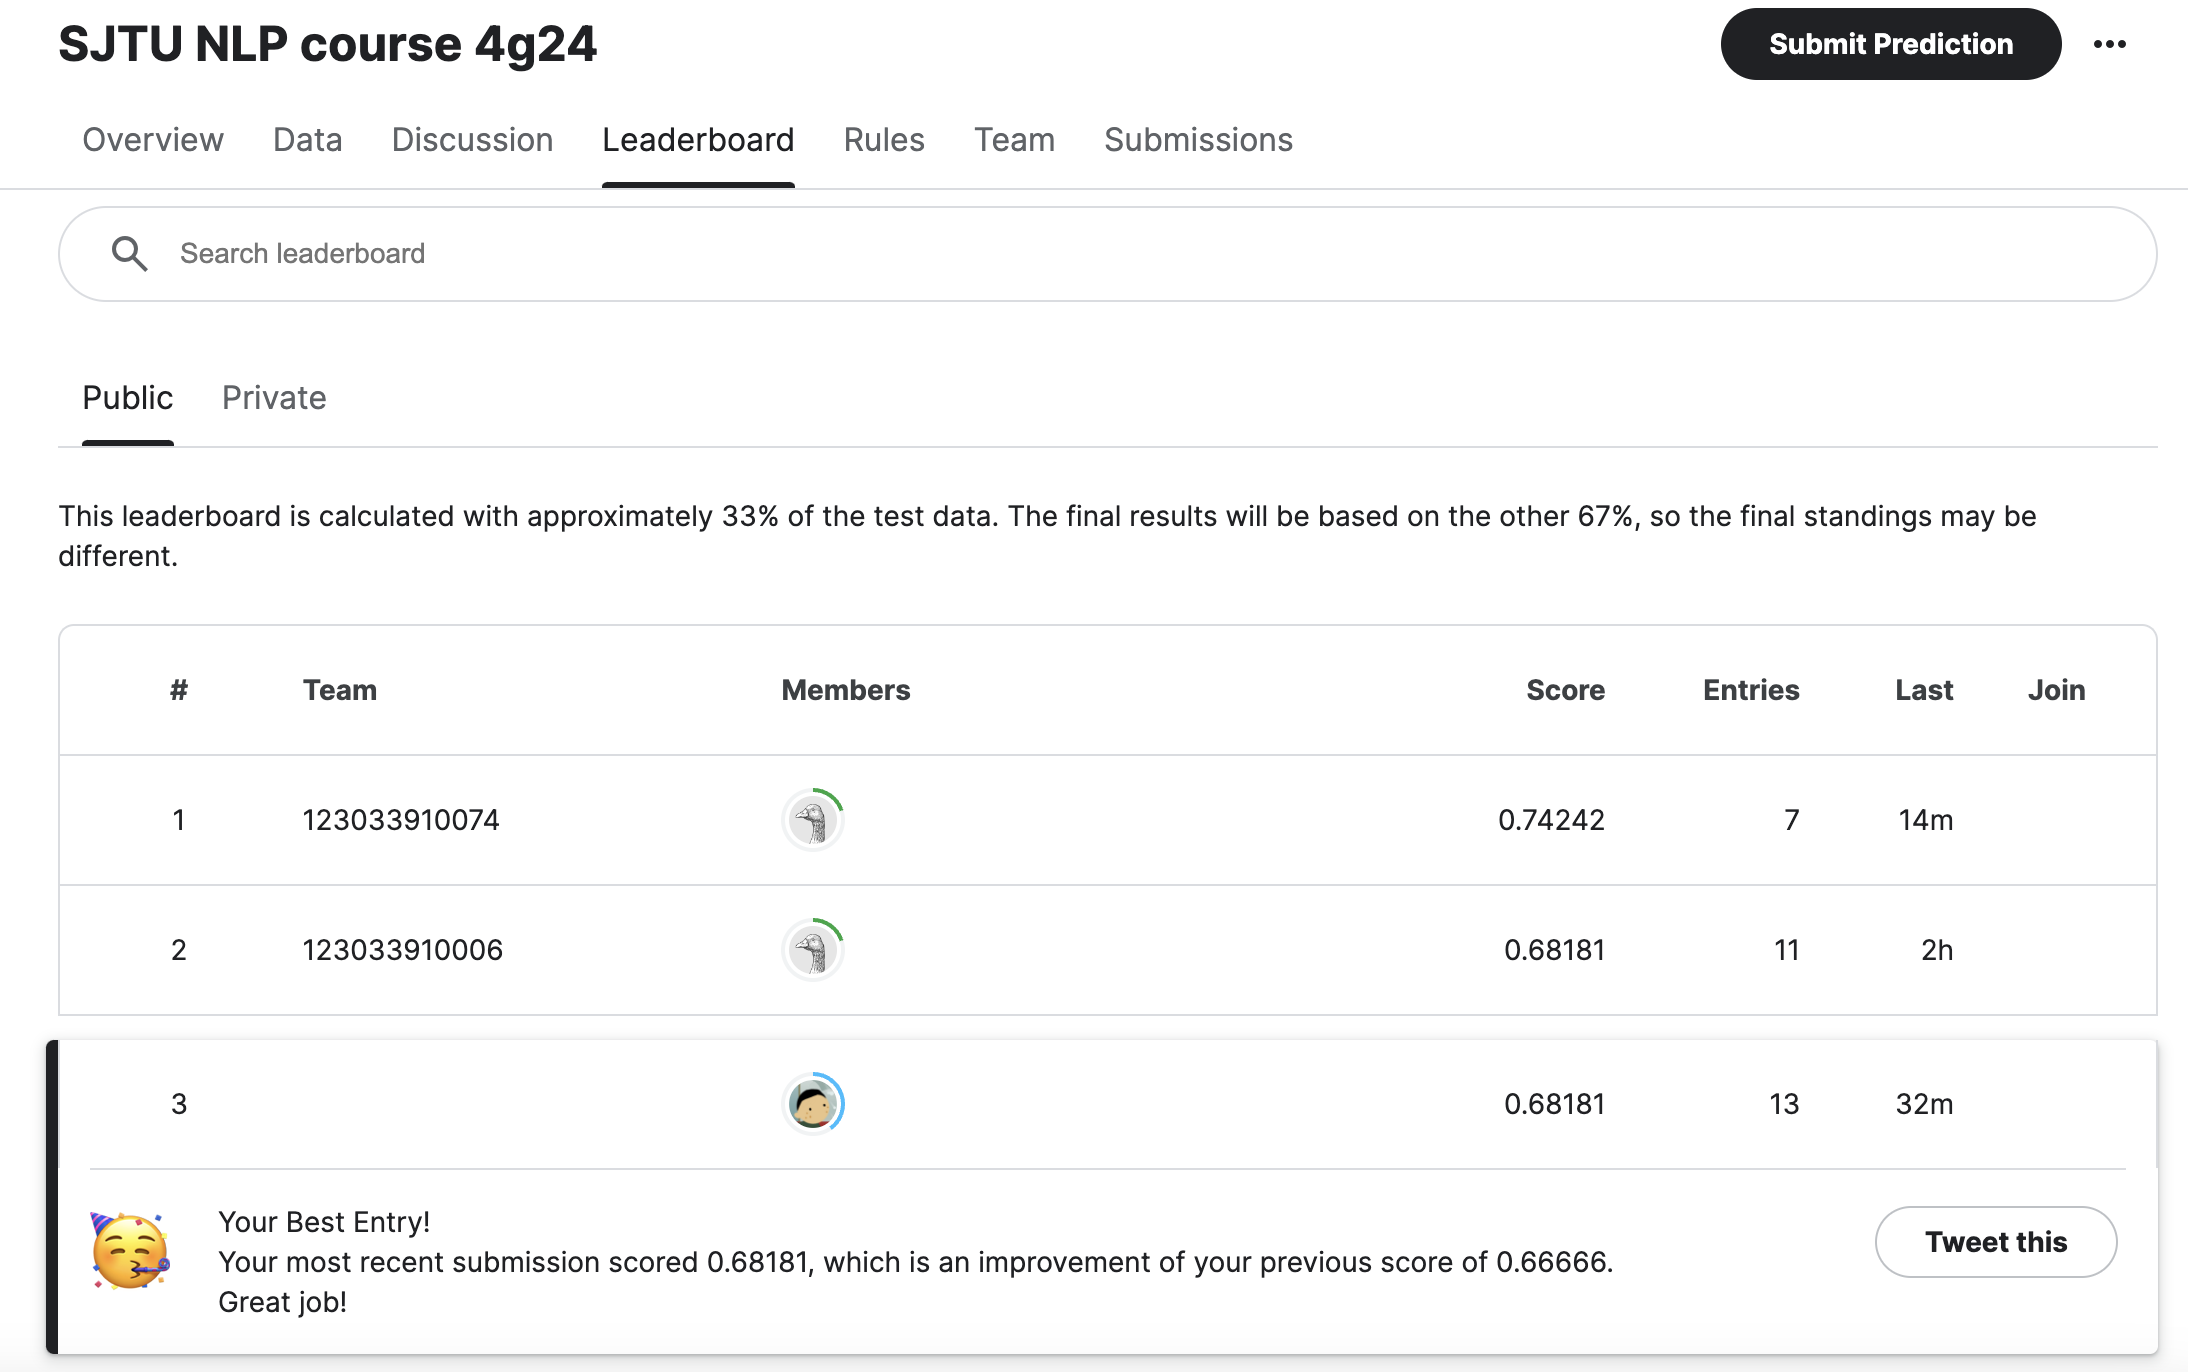
\includegraphics[width=\textwidth]{kaggle.png}
    \caption{Kaggle 结果(2023-05-25)}
    \label{fig:kaggle}
\end{figure}

\printbibliography[heading=bibintoc]

\appendix

\markdownInput{../README.md}

\end{document}